\documentclass[12pt,a4paper,twoside,openright]{report}
\let\openright=\cleardoublepage



%%% Choose a language %%%

\newif\ifEN
\ENtrue   % uncomment this for english
%\ENfalse   % uncomment this for czech

%%% Configuration of the title page %%%

\newif\ifMFF
\MFFtrue % comment this out for the version with a big UK university logo
\def\UKName{Charles University in Prague} %this is only used in UK-logo-version
\def\UKFaculty{Faculty of Mathematics and Physics}

% Thesis type names, as used in several places in the title
\def\ThesisTypeTitle{\ifEN BACHELOR THESIS \else BAKALÁŘSKÁ PRÁCE \fi}
%\def\ThesisTypeTitle{\ifEN MASTER THESIS \else DIPLOMOVÁ PRÁCE \fi}
%\def\ThesisTypeTitle{\ifEN RIGOROUS THESIS \else RIGORÓZNÍ PRÁCE \fi}
%\def\ThesisTypeTitle{\ifEN DOCTORAL THESIS \else DISERTAČNÍ PRÁCE \fi}
\def\ThesisGenitive{\ifEN bachelor \else bakalářské \fi}
%\def\ThesisGenitive{\ifEN master \else diplomové \fi}
%\def\ThesisGenitive{\ifEN rigorous \else rigorózní \fi}
%\def\ThesisGenitive{\ifEN doctoral \else disertační \fi}
\def\ThesisAccusative{\ifEN bachelor \else bakalářskou \fi}
%\def\ThesisAccusative{\ifEN master \else diplomovou \fi}
%\def\ThesisAccusative{\ifEN rigorous \else rigorózní \fi}
%\def\ThesisAccusative{\ifEN doctoral \else disertační \fi}



%%% Fill in your details %%%

% (Note: \xxx is a "ToDo label" which makes the unfilled visible. Remove it.)
\def\ThesisTitle{Modern evolutionary strategies for reinforcement learning problems}
\def\ThesisAuthor{Michal Pospěch}
\def\YearSubmitted{2021}

% department assigned to the thesis
\def\Department{Department of Theoretical Computer Science and Mathematical Logic}
% Is it a department (katedra), or an institute (ústav)?
\def\DeptType{Department}

\def\Supervisor{Mgr. Roman Neruda, CSc.}
\def\SupervisorsDepartment{Department of Theoretical Computer Science and Mathematical Logic}

% Study programme and specialization
\def\StudyProgramme{Computer science}
\def\StudyBranch{General computer science}

\def\Dedication{%
Dedication. \xxx{It is nice to say thanks to supervisors, friends, family, book authors and food providers.}
}

\def\AbstractEN{%
Evolutionary strategies are one of many approaches to solving reinforcement learning tasks. This thesis explores two modern approaches based on them, OpenAI-ES and NS-ES (and its extensions) which utilises novelty search. They are being studied on two environments, Cartpole-swingup and Slimevolley. On Cartpole-swingup they all have some success while performance on Slimevolley is really sensitive to initial seed.
}

\def\AbstractCS{%
Evoluční strategie jsou jeden z přístupů k řešení úloh zpětnovazebného učení. V této práci jsou zkoumány dva moderní přístupy na nich založení, OpenAI-ES a NS-ES (a jeho rozšíření), který využívá hledání novosti. Jsou zkoumány na dvou prostředích, Cartpole-swingup a Slimevolley. Na Cartpole-swingup mají nějaký úspěch všechny, na Slimevolley je chování silně citlivé na úvodní seed.
}

% 3 to 5 keywords (recommended), each enclosed in curly braces.
% Keywords are useful for indexing and searching for the theses by topic.
\def\Keywords{%
{evolutionary strategies} {reinforcement learning} {novelty search} {neuroevolution}
}

% If your abstracts are long and do not fit in the infopage, you can make the
% fonts a bit smaller by this setting. (Also, you should try to compress your abstract more.)
% Alternatively, consider increasing the size of the page by uncommenting the
% geometry modification in thesis.tex.
\def\InfoPageFont{}
%\def\InfoPageFont{\small}  %uncomment to decrease font size

\ifEN\relax\else
% If you are writing a czech thesis, you additionally need to fill in the
% english translation of the metadata here!
\def\ThesisTitleEN{\xxx{Thesis title in English}}
\def\DepartmentEN{\xxx{Name of the department in English}}
\def\DeptTypeEN{\xxx{Department}}
\def\SupervisorsDepartmentEN{\xxx{Superdepartment}}
\def\StudyProgrammeEN{\xxx{study programme}}
\def\StudyBranchEN{\xxx{study branch}}
\def\KeywordsEN{%
\xxx{{key} {words}}
}
\fi


\usepackage[a-2u]{pdfx}

\ifEN\else\usepackage[czech,shorthands=off]{babel}\fi
\usepackage[utf8]{inputenc}
\usepackage[T1]{fontenc}

% See https://en.wikipedia.org/wiki/Canons_of_page_construction before
% modifying the size of printable area. LaTeX defaults are great.
% If you feel it would help anything, you can enlarge the printable area a bit:
%\usepackage[textwidth=390pt,textheight=630pt]{geometry}
% The official recommendation expands the area quite a bit (looks pretty harsh):
%\usepackage[textwidth=145mm,textheight=247mm]{geometry}

%%% FONTS %%%
\usepackage{lmodern} % TeX "original" (this sets up the latin mono)

% Optionally choose an override for the main font for typesetting
\usepackage[mono=false]{libertinus} % popular for comp-sci (ACM uses this)
%\usepackage{tgschola} % Schoolbook-like (gives a bit of historic feel)
%\usepackage[scale=0.96]{tgpagella} % Palladio-like (popular in formal logic).

% Optionally choose a custom sans-serif fonts (e.g. for figures and tables).
% Default sans-serif font is usually Latin Modern Sans. Some font packages
% (e.g. libertinus) replace that with a better matching sans-serif font.
%\usepackage{tgheros} % recommended and very readable (Helvetica-like)
%\usepackage{FiraSans} % looks great
% DO NOT typeset the main text in sans-serif font!
% The serifs make the text easily readable on the paper.

% IMPORTANT FONT NOTE: Some fonts require additional PDF/A conversion using
% the pdfa.sh script. These currently include only 'tgpagella'; but various
% other fonts from the texlive distribution need that too (mainly the Droid
% font family).


% some useful packages
\usepackage{amsmath,amsfonts,amsthm,bm}
\usepackage{graphicx}
\usepackage{xcolor}
\usepackage{booktabs}
\usepackage{caption}
\usepackage{floatrow}

% load bibliography tools
\usepackage[backend=bibtex,natbib,style=numeric,sorting=none]{biblatex}
% alternative with alphanumeric citations (more informative than numbers):
%\usepackage[backend=bibtex,natbib,style=alphabetic]{biblatex}
%
% alternatives that conform to iso690
% (iso690 is not formally required on MFF, but may help elsewhere):
%\usepackage[backend=bibtex,natbib,style=iso-numeric,sorting=none]{biblatex}
%\usepackage[backend=bibtex,natbib,style=iso-alphabetic]{biblatex}
%
% additional option choices:
%  - add `giveninits=true` to typeset "E. A. Poe" instead of full Edgar Allan
%  - `terseinits=true` additionaly shortens it to nature-like "Poe EA"
%  - add `maxnames=10` to limit (or loosen) the maximum number of authors in
%    bibliography entry before shortening to `et al.` (useful when referring to
%    book collections that may have hundreds of authors)
%  - for additional flexibility (e.g. multiple reference sections, etc.),
%    remove `backend=bibtex` and compile with `biber` instead of `bibtex` (see
%    Makefile)
%  - `sorting=none` causes the bibliography list to be ordered by the order of
%    citation as they appear in the text, which is usually the desired behavior
%    with numeric citations. Additionally you can use a style like
%    `numeric-comp` that compresses the long lists of citations such as
%    [1,2,3,4,5,6,7,8] to simpler [1--8]. This is especially useful if you plan
%    to add tremendous amounts of citations, as usual in life sciences and
%    bioinformatics.
%  - if you don't like the "In:" appearing in the bibliography, use the
%    extended style (`ext-numeric` or `ext-alphabetic`), and add option
%    `articlein=false`.
%
% possibly reverse the names of the authors with the default styles:
%\DeclareNameAlias{default}{family-given}

% load the file with bibliography entries
\addbibresource{refs}

% remove this if you won't use fancy verbatim environments
\usepackage{fancyvrb}

% remove this if you won't typeset TikZ graphics
\usepackage{tikz}
\usetikzlibrary{positioning} %add libraries as needed (shapes, decorations, ...)

% remove this if you won't typeset any pseudocode
\usepackage{algpseudocode}
\usepackage{algorithm}

% remove this if you won't list any source code
\usepackage{listings}


\hypersetup{unicode}
\hypersetup{breaklinks=true}

\usepackage[noabbrev]{cleveref}


% various forms of TODOs (you should remove this before submitting)
\usepackage[textsize=tiny, backgroundcolor=yellow!25, linecolor=black!25]{todonotes}
\newcommand{\xxx}[1]{\textcolor{red!}{#1}}

 % remove this before compiling the final version


% use this for typesetting a chapter without a number, e.g. intro and outro
\def\chapwithtoc#1{
\chapter*{#1}
\addcontentsline{toc}{chapter}{#1}
}

% If there is a line/figure overflowing into page margin, this will make the
% problem evident by drawing a thick black line at the overflowing spot. You
% should not disable this.
\overfullrule=3mm

% The maximum stretching of a space. Increasing this makes the text a bit more
% sloppy, but may prevent the overflows by moving words to next line.
\emergencystretch=1em

\ifEN
\theoremstyle{plain}
\newtheorem{thm}{Theorem}
\newtheorem{lemma}[thm]{Lemma}
\newtheorem{claim}[thm]{Claim}
\newtheorem{defn}{Definition}
\theoremstyle{remark}
\newtheorem*{cor}{Corollary}
\else
\theoremstyle{plain}
\newtheorem{thm}{Věta}
\newtheorem{lemma}{Lemma}
\newtheorem{claim}{Tvrzení}
\newtheorem{defn}{Definice}
\theoremstyle{remark}
\newtheorem*{cor}{Důsledek}
\fi

\newenvironment{myproof}{
  \par\medskip\noindent
  \textit{\ifEN Proof \else Důkaz \fi}.
}{
\newline
\rightline{$\qedsymbol$}
}

% real/natural numbers
\newcommand{\R}{\mathbb{R}}
\newcommand{\N}{\mathbb{N}}

% asymptotic complexity
\newcommand{\asy}[1]{\mathcal{O}(#1)}

% listings and default lstlisting config (remove if unused)
\DeclareNewFloatType{listing}{}
\floatsetup[listing]{style=ruled}

\DeclareCaptionStyle{thesis}{style=base,font={small,sf},labelfont=bf,labelsep=quad}
\captionsetup{style=thesis}
\captionsetup[algorithm]{style=thesis,singlelinecheck=off}
\captionsetup[listing]{style=thesis,singlelinecheck=off}

\ifEN\floatname{listing}{Listing}
\else\floatname{listing}{Výpis kódu}\fi
\lstset{%
  language=C++,
  tabsize=2,
  showstringspaces=false,
  basicstyle=\footnotesize\tt\color{black!75},
  identifierstyle=\bfseries\color{black},
  commentstyle=\color{green!50!black},
  stringstyle=\color{red!50!black},
  keywordstyle=\color{blue!75!black}}

% Czech versions of the used cleveref references (It's not as convenient as in
% English because of declension, cleveref is limited to sg/pl nominative. Use
% plain \ref to dodge that.)
\ifEN\relax\else
\crefname{chapter}{kapitola}{kapitoly}
\Crefname{chapter}{Kapitola}{Kapitoly}
\crefname{section}{sekce}{sekce}
\Crefname{section}{Sekce}{Sekce}
\crefname{subsection}{sekce}{sekce}
\Crefname{subsection}{Sekce}{Sekce}
\crefname{subsubsection}{sekce}{sekce}
\Crefname{subsubsection}{Sekce}{Sekce}
\crefname{figure}{obrázek}{obrázky}
\Crefname{figure}{Obrázek}{Obrázky}
\crefname{table}{tabulka}{tabulky}
\Crefname{table}{Tabulka}{Tabulky}
\crefname{listing}{výpis}{výpisy}
\Crefname{listing}{Výpis}{Výpisy}
\floatname{algorithm}{Algoritmus}
\crefname{algorithm}{algoritmus}{algoritmy}
\Crefname{algorithm}{Algoritmus}{Algoritmy}
\newcommand{\crefpairconjunction}{ a~}
\newcommand{\crefrangeconjunction}{ a~}
\fi
 % use this file for various custom definitions


\begin{document}

% the layout is mandatory, edit only in dire circumstances

\pagestyle{empty}
\hypersetup{pageanchor=false}
\begin{center}

\ifMFF
\ifEN
\centerline{\mbox{
\includegraphics[width=166mm]{img/logo-en.pdf}}}
\else
\centerline{\mbox{
\includegraphics[width=166mm]{img/logo-cs.pdf}}}
\fi
\vspace{-8mm}
\else
{\large\noindent\UKName\par\medskip\par\UKFaculty }
\fi
\vfill

{\bf\Large\ThesisTypeTitle}

\vfill

\ifMFF\relax\else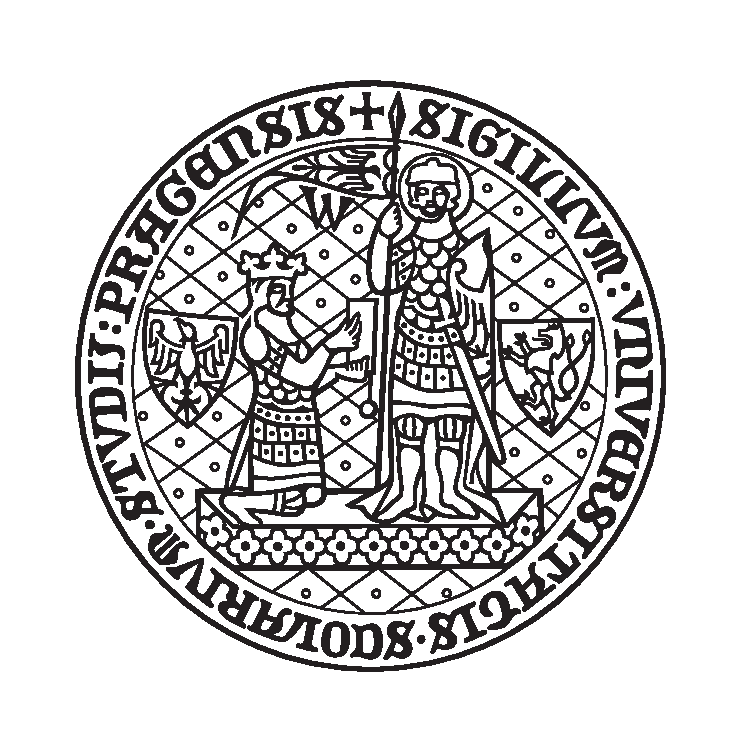
\includegraphics[width=70mm]{img/uklogo.pdf}

\vfill\fi

{\LARGE\ThesisAuthor}

\vspace{15mm}

{\LARGE\bfseries\ThesisTitle}

\vfill

\Department

\vfill

{
\centerline{\vbox{\halign{\hbox to 0.45\hsize{\hfil #}&\hskip 0.5em\parbox[t]{0.45\hsize}{\raggedright #}\cr
\ifEN Supervisor of the \ThesisGenitive thesis:
\else Vedoucí \ThesisGenitive práce: \fi
& \Supervisor \cr
\noalign{\vspace{2mm}}
\ifEN Study programme: \else Studijní program: \fi
& \StudyProgramme \cr
\noalign{\vspace{2mm}}
\ifEN Study branch: \else Studijní obor: \fi
& \StudyBranch \cr
}}}}

\vfill

\ifEN Prague \else Praha \fi
\YearSubmitted

\end{center}

\newpage

% remember to sign this!
\openright
\hypersetup{pageanchor=true}
\pagestyle{plain}
\pagenumbering{roman}
\vglue 0pt plus 1fill

\ifEN
\noindent
I declare that I carried out this \ThesisAccusative thesis independently, and only with the cited
sources, literature and other professional sources. It has not been used to obtain another
or the same degree.
\else
\noindent
Prohlašuji, že jsem tuto \ThesisAccusative práci vypracoval(a) samostatně a výhradně
s~použitím citovaných pramenů, literatury a dalších odborných zdrojů.
Tato práce nebyla využita k získání jiného nebo stejného titulu.
\fi

\ifEN
\medskip\noindent
I understand that my work relates to the rights and obligations under the Act No.~121/2000 Sb.,
the Copyright Act, as amended, in particular the fact that the Charles
University has the right to conclude a license agreement on the use of this
work as a school work pursuant to Section 60 subsection 1 of the Copyright~Act.
\else
\medskip\noindent
Beru na~vědomí, že se na moji práci vztahují práva a povinnosti vyplývající
ze zákona č. 121/2000 Sb., autorského zákona v~platném znění, zejména skutečnost,
že Univerzita Karlova má právo na~uzavření licenční smlouvy o~užití této
práce jako školního díla podle §60 odst. 1 autorského zákona.
\fi

\vspace{10mm}


\ifEN
\hbox{\hbox to 0.5\hsize{%
In \hbox to 6em{\dotfill} date \hbox to 6em{\dotfill}
\hss}\hbox to 0.5\hsize{\dotfill\quad}}
\smallskip
\hbox{\hbox to 0.5\hsize{}\hbox to 0.5\hsize{\hfil Author's signature\hfil}}
\else
\hbox{\hbox to 0.5\hsize{%
V \hbox to 6em{\dotfill} dne \hbox to 6em{\dotfill}
\hss}\hbox to 0.5\hsize{\dotfill\quad}}
\smallskip
\hbox{\hbox to 0.5\hsize{}\hbox to 0.5\hsize{\hfil Podpis autora\hfil}}
\fi

\vspace{20mm}
\newpage

% dedication

\openright

\noindent
\Dedication

\newpage

% mandatory information page

\openright

\vbox to 0.49\vsize{\InfoPageFont
\setlength\parindent{0mm}
\setlength\parskip{5mm}

\ifEN Title: \else Název práce: \fi
\ThesisTitle

\ifEN Author: \else Autor: \fi
\ThesisAuthor

\DeptType:
\Department

\ifEN Supervisor: \else Vedoucí bakalářské práce: \fi
\Supervisor, \SupervisorsDepartment

\ifEN Abstract: \AbstractEN \else Abstrakt: \AbstractCS \fi

\ifEN Keywords: \else Klíčová slova: \fi
\Keywords

\vss}\ifEN\relax\else\nobreak\vbox to 0.49\vsize{\InfoPageFont
\setlength\parindent{0mm}
\setlength\parskip{5mm}

Title:
\ThesisTitleEN

Author:
\ThesisAuthor

\DeptTypeEN:
\DepartmentEN

Supervisor:
\Supervisor, \SupervisorsDepartmentEN

Abstract:
\AbstractEN

Keywords:
\KeywordsEN

\vss}
\fi

\newpage

\openright
\pagestyle{plain}
\pagenumbering{arabic}
\setcounter{page}{1}


\tableofcontents


\chapwithtoc{Introduction}


\chapter{Theoretical background}


\section{Reinforcement learning}
\label{sec:reinf}
The key problem that reinforcement learning is trying to solve is controlling an \emph{agent} in an \emph{environment}. The agent interacts with the environment by selecting some action and the environment responds by presenting the agent with a new situation. The environment also provides a numerical reward to the agent whose task is to maximise it over time.

More formally, the agent interacts with the environment in discrete (if the problem has continuous time, it is discretised) time steps $t=1,2,3,\dots$. At each time step the agent recieves $S_t\in\mathcal{S}$, a representation of internal state of the environment. Based on that it selects an action $A_t\in\mathcal{A}$. This results in the agent receiving a reward $R_{t+1}\in \mathcal{R}\subset \mathbb{R}$ in addition to a new state $S_{t+1}$ in the next step generating a sequence or \emph{trajectory} beginning like this:
\begin{equation}
    S_0,A_0,R_1,S_1,A_1,R_2,S_2,A_2,R_3,\dots
\end{equation}
The random variables $S_t$ and $R_t$ depend only on the preceding state and action based on function $p: \mathcal{S} \times \mathcal{R} \times \mathcal{S} \times\mathcal{A} \rightarrow [0,1]$ characterising \emph{dynamics} of the problem with following definition:
\begin{equation}
    p(s',r|s,a) = \text{Pr}\{S_t=s',R_t=r|S_{t-1}=s, A_{t-1}=a\}.
\end{equation}
This can, however, be viewed as an restriction on information contained in state rather than restriction on the environment. If the state does contain all information that influence the future then it has the \emph{Markovian property} and the problem at hand is a \emph{Markov decision process}.

To formally describe what is the goal of reinforcement learning \emph{expected return} $G_t$ needs to be defined first. It is a function of the reward sequence, in the simplest case an ordinary sum of rewards 
\begin{equation}
    \label{eq:exp-ret}
    G_t = \sum_{i=t+1}^TR_i,
\end{equation}
where $T$ is the final time step. 

This approach works only if the there is a final step in the interaction which would divide the interaction into subsequences called \emph{episodes}. Each episodes ends when the environment reaches a \emph{terminal state} and is reset into its initial state afterwards.
Such tasks are called \emph{episodic tasks}. 

Contrary to that there are tasks which do not break into episodes, they continue indefinitely. They are called \emph{continuing tasks} For these the definition \ref{eq:exp-ret} doesn't work as the sum could possibly be infinite. To calculate expected reward for such tasks a modified approach is needed. A \emph{discount rate} $\gamma \in [0,1]$ is introduced to define \emph{discounted return}
\begin{equation}
    \label{eq:disc-ret}
    G_t = \sum_{i=0}^\infty \gamma^iR_{t+i+1}.
\end{equation}
The discount rate makes future reward worth less at the moment of decision. If $\gamma<1$ and the reward are bounded, then the infinite sum \ref{eq:disc-ret} is finite. For $\gamma=0$ the agent is said to be "myopic" taking into account only the immediate reward and ignoring the future. Otherwise as $\gamma$ approaches $1$ the future rewards have bigger weight and influence the agent's decision more.
Succesive returns are related in a way

A common occurence in reinforcement learning is an estimating \emph{value function} which estimate how beneficial it is for the agent to be in that state. This is defined by the expected return which is dependent on the actions that the agent will perform. Therefore a value function must be defined with respect to such way of acting called \emph{policy}.

Policy is a function $\pi: \mathcal{S} \times \mathcal{A} \rightarrow [0,1]$ returning probability of selecting each action in given state meaning that agent following policy $\pi$ at time $t$ would select action $A_t = a$ if in state $S_t =s$ with probability $\pi(a|s)$. The policy function is changed by reinforcement learning based on the agent's experience.

For state $s$ and policy $\pi$ the \emph{state-value function} $v_\pi(s)$ gives the expected return when starting in state $s$ and following policy $\pi$, formally (for MDPs)
\begin{equation}
    v_\pi(s) = \mathrm{E}_\pi[G_t|S_t=s],
\end{equation}
where $\mathrm{E}_\pi[.]$ is expected value when following policy $\pi$ in every timestep. 

\emph{Action-value function} $q_\pi(s,a)$ for policy $\pi$ is defined similarly. It gives the expeted return of taking action $a$ in state $s$ while following policy $\pi$, formally
\begin{equation}
    q_\pi(s,a) = \mathrm{E}_\pi[G_t|S_t=s, A_t=a].
\end{equation}\cite{Sutton1998}
\subsection{Methods}
Methods of reinforcement learning can be divided into 3 categories: \begin{itemize}
    \item classical (tabular),
    \item policy gradient-based and
    \item evolutionary.
\end{itemize}

Classical methods rely on updating \emph{Q-values} for each state-action pair therefore they require having discrete sets of actions and states. Based on the Q-values a policy is derived, such as an $\varepsilon$-greedy policy which (in training) chooses a random action with probability $\varepsilon$ and the currently best action in all other cases. One of the most well known algorithms is \emph{Q-learning}. In it the Q-values are updated each step via following formula:
\begin{equation}
    q(s_t,a_t) = q(s_t,a_t) + \alpha \left( r_t+\gamma \max_a q(s_{t-1},a)-q(s_t,a_t)\right), 
\end{equation}
where $\alpha$ is the learning rate.

\begin{algorithm}[h]
    \begin{algorithmic}[1]
    \caption{Q-Learning}
    \label{alg:q-learning}
        \State parameters: learning rate $\alpha \in (0,1]$ 
        \State initialise: $q(s,a)$ for all $s\in\mathcal{S}$ and $a\in \mathcal{A}$ arbitrarily, except for $q(terminal, \cdot) = 0$ 
        \For{each episode}
            \State initialise $s\in\mathcal{S}$
            \Repeat
                \State choose $a$ from $s$ using policy derived from $q$
                \State take action $a$, observe $s', r$
                \State $q(s,a) = q(s,a) + \alpha \left( r+\gamma \max_a q(s',a)-q(s,a)\right)$
                \State $s = s'$
            \Until{$s$ is terminal state}
        \EndFor
    \end{algorithmic}
\end{algorithm}

Policy-gradient based methods are methods that utilise the gradient in policy space. They are one  of the few optimisation strategies able to handle reinforcement learning tasks that are high-dimensional and have continuous state and action space. One of the most known algorithms from this group is \emph{REINFORCE}.
\begin{algorithm}[h]
    \begin{algorithmic}[1]
    \caption{REINFORCE}
    \label{alg:reinforce}
        \State parameters: step size $\alpha>0$ 
        \State input: differentiable policy parametrisation $\pi(a|s,\theta)$
        \State initialise: policy parameters $\theta$ atrbitrarily
        \For{each episode}
            \State generate $S_0, A_0, R_1,\dots,S_{T-1},A_{T-1},R_T$ by following $\pi(\cdot|\cdot,\theta)$
            \For{each timestep $t \in \{0,1,\dots, T-1\}$}
                \State $G = \sum_{k=t+1}^T\gamma^{k-t-1}R_k$
                \State $\theta = \theta + \alpha \gamma^t G \nabla\ln\pi(A_t,S_t,\theta)$
            \EndFor
        \EndFor
    \end{algorithmic}
\end{algorithm}


Another, not as known, class of policy-gradient based algorithms are PEPG (Parameter exploring policy gradient).\cite{Sehnke2012} They use samples from parameter space to estimate the log-likelyhood on parameter level. In traditional policy gradient methods the policy is probabilistic, it returns a distribution from which the next action is selected and final gradient is calculated by differentiating the policy with respect to parameters. This however causes high variance in samples over more episodes thus a noisy gradient estimate. PEPG circumvent this issue by having a probability distribution over policy parameters with a deterministic policy.


\begin{algorithm}[h]
    \begin{algorithmic}[1]
    \caption{PGPE (Policy Gradients with Parameter-based Exploration) with symmetric sampling}
    \label{alg:pgpe}
        \State parameters: step size $\alpha>0$, number of histories $n$ 
        \State initialise: $\mu, \sigma$ (both $n$ dimensional) to preselected initial values, $m=0$
        \Repeat
            \For{$i \in {1,\dots,n}$}
                \State sample $\epsilon^i \sim \mathcal{N}(0,I\sigma^2)$
                \State $\theta^+ = \mu+\epsilon^i$
                \State $\theta^- = \mu-\epsilon^i$
                \State evaluate policies $\pi(\cdot|\cdot,\theta^+)$ and $\pi(\cdot|\cdot, \theta^-)$ and get rewards $r^{+i}, r^{-i}$
                
            \EndFor
            \State Set matrix $T$ as $T_{ij} = \epsilon_i^j$
            \State Set matrix $S$ as $S_{ij} = \frac{(\epsilon^j_i)^2-\sigma_i^2}{\sigma_i}$
            \State $r_T = [(r^{+1}-r^{-1}),\dots,(r^{+n}-r^{-n})]^T$
            \State $r_S = [\frac{(r^{+1}+r^{-1})}{2},\dots,\frac{(r^{+n}+r^{-n})}{2}]^T$
            \State Update $\mu = \mu + \alpha T r_T$
            \State Update $\sigma = \sigma + \alpha S r_S$
            \Until{stop criterion is fullfilled}
    \end{algorithmic}
\end{algorithm}


Evolutionary methods utilise only \emph{fitness} describing the overall performance of the agent. Exploration is done via changing parameters that influence the agent's behaviour. However the basis of this class of algorithms is not derived from the mathematical principles of reinfocement learning. They are further described in following chapters.

\section{Evolutionary algorithms}
\label{sec:ea}
Evolutionary algorithms (EA) are a type of optimisation metaheuristics inspired by the process of bilogical evolution. At first a number of possible solutions to the problem at hand is generated (\emph{population}) and each solution (\emph{individual}) is encoded (via a domain-specific encoding) and evaluated giving us the value of its \emph{fitness}. Fitness is a function describing how good that particular individual is and it is everything that is needed for creation of  Then a new population is created using a \emph{crossover} (combination) of 1 or more individuals which are selected using the operator of \emph{parental selection}. Each of the newly created individuals has a chance to be mutated via the \emph{mutation} operator. Finally a new population is selected from \emph{offsprings} and possibly the parents based of fitness and enters the next iteration of the EA and the following generation is chosen using \emph{environmental selection} operator. The algorithm repeats until the stop condition is met, usually a set number of iterations or small improvement of fitness between 2 generations. 

There are many variands of EAs such as genetic algorithms (most common), genetic programming, evolutionary programming, neuroevolution or evolutionary strategies that are further described in following chapter. \cite{Rudolph2012} \cite{Vikhar2016}

\begin{algorithm}[h]
    \begin{algorithmic}[1]
    \caption{Evolutionary algorithm}\label{alg:ea}
        \State initialize population $P^0$ with $n$ individuals
        \State set $t=0$
        \Repeat
            \State $Q^t = \{\}$
            \For{$i \in \{1\dots m\}$}
                \State $p_1,\dots,p_\rho = ParentalSelection(P^t)$
                \State $q = Crossover(p_1,\dots,p_\rho)$ 
                \State $q = Mutation(q)$ with chance $p$
                \State $Q^t = q \cup Q^t$
            \EndFor
            \State $P^{t+1} =EnvironmentalSelection(Q^t\cup  P^t)$
            \State increment $t$
        \Until{stop criterion fullfilled}
    \end{algorithmic}
    \end{algorithm}

\section{Evolutionary strategies}
\label{sec:es}
Evolutionary strategies (ES) are a type of optimisation metaheuristic which further specialises EA and restricts their level of freedom. The selection for crossover is unbiased, mutation is parametrised and thus controllable, individuals which should be put to next generation are chosen ordinally based on fitness and individuals contain not only the problem solution but also control parameters.

More formally ES $(\mu / \rho,\kappa,\lambda)$ has $\mu$ individuals in each generation, which produces $\lambda$ offsprings, each created by crossover of $\rho$ individuals and each individual is able to survive for up to $\kappa$ generations as described in algorithm \ref{alg:es}. This notation further generalizes the old $(\mu,\lambda)$ and $(\mu+\lambda)$ notations, where the "," notation means $\kappa=1$ and "+" notation $\kappa=\infty$. 
\begin{algorithm}[h]
\begin{algorithmic}[1]
\caption{$(\mu / \rho,\kappa,\lambda)$-ES}
\label{alg:es}
    \State initialize population $P^0$ with $\mu$ individuals
    \State set age for each $p\in P^0$ to $1$
    \State set $t=0$
    \Repeat
        \State $Q^t = \{\}$
        \For{$i \in \{1\dots\lambda\}$}
            \State select $\rho$ parents $p_1,\dots,p_\rho \in P^t$ uniformly at random
            \State $q = variation(p_1,\dots,p_\rho)$ with age $0$
            \State $Q^t = q \cup Q^t$
        \EndFor
        \State $P^{t+1} =$ select $\mu$ best (wrt. fitness) individuals from $Q^t\cup \{p \in P^t: age(p)<\kappa\}$
        \State increment age by 1 for each $p \in P^{t+1}$
        \State increment $t$
    \Until{stop criterion fullfilled}
\end{algorithmic}
\end{algorithm}

To design an ES one must first select an appropriate representation for an individual and the most natural one is prefered in most cases, if all parameters are of one type (e.g. a real number) a simple vector will suffice, if the types are mixed, a tuple of vectors is required. This however causes an increased complexity of the variation operator.

As for design of the variation operator there are some guidelines that should be followed when designing it.
\begin{description}
    \item[Reachability] every solution should be reachable from any other solution in a finite number of applications of the variation operator with probability $p > 0$
    \item[Unbiasedness] the operator should not favour any particular subset of solution unless provided with information about problem at hand
    \item[Control] the operator should be parametrised in such way that the size of the distribution can be controlled (practice had shown that decreasing it as the optimal solution is being approached is necessary) 
\end{description}

A big part of designing efficient evolutionary strategy algorithms is adapting the covariance matrix of the used multivariate normal distribution that is commonly used as variation operator. It is assumed that setting the covariance matrix $\Sigma$ of the distribution proportional to the inverse Hessian matrix of Taylor expansion of the fitness function. This would align the hyperellipsoid of equal probabilities of the mutation distribution with the hyperellipsoid of equal fitness values.\cite{Schwefel1995}\cite{Rudolph2012}

\subsection{CMA-ES}
\label{subsec:cma-es}
The aforementioned idea is used in Covariance Matrix Adaptation Evolutionary Strategy algorithm. In it the population of new individuals is generated by sampling a multivariate normal distribution. The individuals are sampled via following equation for generation $t \in \mathrm{N}_0$:
\begin{equation}
    x_k^{t+1} \sim m^t + \sigma^t\mathcal{N}(0,C^t),\ k\in \{1,2,\dots,\lambda\}, 
\end{equation}
where 
\begin{description}
    \item $x_k^{t+1}$ is $k$-th individual from generation $t+1$, 
    \item $m^t$ is mean value of the search distribution at generation $t$,
    \item $\sigma^t$ is the step size at generation $t$,
    \item $C^t$ is the covariance matrix at generation $t$ and
    \item $\lambda$ is the population size.
\end{description}

At each step the mean is moved to the weighted average of $\mu$ selected individuals (parents) from the current generation. The individuals are selected based on their fitness and the weights are parameters of the algorithm. Then the covariance matrix $C^t$ is updated using the covariance matrix from previous generation, the evolution steps and the new individuals. To control the step size $\sigma^t$ only information from evolution steps is used.\cite{hansen2016cma}

\begin{algorithm}[h]
    \begin{algorithmic}[1]
    \caption{CMA-ES}
    \label{alg:cma-es}
        \State parameters: $\lambda, w_{i=1\dots\lambda}, c_\sigma,d_\sigma, c_c, c_\mu$ (set according to Table 1 in \cite{hansen2016cma})
        \State initialise: $p_\sigma=0,p_c=0$, covariance matrix $C=I$, $g=0$, distribution mean $m$ and $\sigma > 0$ step-size depending on the problem
        \State set $t=0$
        \Repeat
            \State increment $t$
            \State calculate matrices $B,D$ such that $C=BDDB^T$ (spectral decomposition)
            \For{$ k= 1,\dots,\lambda$}
            \Comment sample new individuals
                \State $z_k \sim \mathcal{N}(0,I)$
                \State $y_k = BDz_k$
                \State $x_k = m+\sigma y_k$
                \State evaluate $x_k$
            \EndFor
            \State $\langle y_t\rangle_w = \sum_{i=1}^\mu w_i y_{y:\lambda} $ \Comment $y_{i:\lambda}$ is $i$-th best performing individual
            \State $m = m+c_m \sigma \langle y\rangle_w$
            \State $p_\sigma = (1-c_\sigma)p_\sigma + \sqrt{c_\sigma (2-c_c)\mu_{\text{eff}}}C^{-\frac{1}{2}}\langle y \rangle_w$ \Comment $\mu_{\text{eff}}=(\sum_{i=1}^\lambda w_i^2)^{-1}$
            \State $\sigma = \sigma \exp(\frac{c_\sigma}{d_\sigma}(\frac{\Vert p_\sigma\Vert}{\mathrm{E}\Vert\mathcal{N}(0,I)\Vert}-1))$
            \State $w_i' = w_i(1\ \text{if}\ w_i> 0\ \text{else}\ n/ \Vert C^{-\frac{1}{2}}y_{i:\lambda}\Vert^2)$
            \State $C = (1+c_1\delta(h_\sigma)-c_1-c_\mu\sum_{i=1}^\lambda w_i)C + c_1p_cp_c^T + c_\mu\sum_{i=1}^\lambda w_i'y_{i:\lambda}y_{i:\lambda}^T$
        \Until{stop criterion fullfilled}
    \end{algorithmic}
    \end{algorithm}

\chapter{Theory}
\label{chap:theory}

\section{Reinforcement learning}
\label{sec:reinf}
\begin{itemize}
    \item problem description (state space, action space, reward...)
    \item various methods \begin{itemize}
        \item value function
        \item criterion of optimality
        \item direct policy search (and various methods)
    \end{itemize}
\end{itemize}
\section{Evolutionary algorithms}
\label{sec:ea}
Evolutionary algorithms (EA) are a type of optimisation metaheuristics inspired by the process of bilogical evolution. At first a number of possible solutions to the problem at hand is generated (\emph{population}) and each solution (\emph{individual}) is encoded (via a domain-specific encoding) and evaluated giving us the value of its \emph{fitness}. Fitness is a function describing how good that particular individual is and it is everything that is needed for creation of  Then a new population is created using a \emph{crossover} (combination) of 1 or more individuals which are selected using the operator of \emph{parental selection}. Each of the newly created individuals has a chance to be mutated via the \emph{mutation} operator. Finally a new population is selected from \emph{offsprings} and possibly the parents based of fitness and enters the next iteration of the EA and the following generation is chosen using \emph{environmental selection} operator. The algorithm repeats until the stop condition is met, usually a set number of iterations or small improvement of fitness between 2 generations. 

There are many variands of EAs such as genetic algorithms (most common), genetic programming, evolutionary programming, neuroevolution or evolutionary strategies that are further described in following chapter. \cite{Rudolph2012} \cite{Vikhar2016}

\begin{algorithm}
    \begin{algorithmic}[1]
    \caption{Evolutionary algorithm}\label{alg:ea}
        \State initialize population $P^0$ with $n$ individuals
        \State set $t=0$
        \Repeat
            \State $Q^t = \{\}$
            \For{$i \in \{1\dots m\}$}
                \State $p_1,\dots,p_\rho = ParentalSelection(P^t)$
                \State $q = Crossover(p_1,\dots,p_\rho)$ 
                \State $q = Mutation(q)$ with chance $p$
                \State $Q^t = q \cup Q^t$
            \EndFor
            \State $P^{t+1} =EnvironmentalSelection(Q^t\cup  P^t)$
            \State increment $t$
        \Until{stop criterion fullfilled}
    \end{algorithmic}
    \end{algorithm}

\section{Evolutionary strategies}
\label{sec:es}
Evolutionary strategies (ES) are a type of optimisation metaheuristic which further specialises EA and restricts their level of freedom. The selection for crossover is unbiased, mutation is parametrised and thus controllable, individuals which should be put to next generation are chosen ordinally based on fitness and individuals contain not only the problem solution but also control parameters.

More formally ES $(\mu / \rho,\kappa,\lambda)$ has $\mu$ individuals in each generation, which produces $\lambda$ offsprings, each created by crossover of $\rho$ individuals and each individual is able to survive for up to $\kappa$ generations as described in algorithm \ref{alg:es}. This notation further generalizes the old $(\mu,\lambda)$ and $(\mu+\lambda)$ notations, where the "," notation means $\kappa=1$ and "+" notation $\kappa=\infty$. 
\begin{algorithm}
\begin{algorithmic}[1]
\caption{$(\mu / \rho,\kappa,\lambda)$-ES}
\label{alg:es}
    \State initialize population $P^0$ with $\mu$ individuals
    \State set age for each $p\in P^0$ to $1$
    \State set $t=0$
    \Repeat
        \State $Q^t = \{\}$
        \For{$i \in \{1\dots\lambda\}$}
            \State select $\rho$ parents $p_1,\dots,p_\rho \in P^t$ uniformly at random
            \State $q = variation(p_1,\dots,p_\rho)$ with age $0$
            \State $Q^t = q \cup Q^t$
        \EndFor
        \State $P^{t+1} =$ select $\mu$ best (wrt. fitness) individuals from $Q^t\cup \{p \in P^t: age(p)<\kappa\}$
        \State increment age by 1 for each $p \in P^{t+1}$
        \State increment $t$
    \Until{stop criterion fullfilled}
\end{algorithmic}
\end{algorithm}

To design an ES one must first select an appropriate representation for an individual and the most natural one is prefered in most cases, if all parameters are of one type (e.g. a real number) a simple vector will suffice, if the types are mixed, a tuple of vectors is required. This however causes an increased complexity of the variation operator.

As for design of the variation operator there are some guidelines that should be followed when designing it.
\begin{description}
    \item[Reachability] every solution should be reachable from any other solution in a finite number of applications of the variation operator with probability $p > 0$
    \item[Unbiasedness] the operator should not favour any particular subset of solution unless provided with information about problem at hand
    \item[Control] the operator should be parametrised in such way that the size of the distribution can be controlled (practice had shown that decreasing it as the optimal solution is being approached is necessary) 
\end{description}
\todo{kovariance}
\cite{Schwefel1995}
\cite{Rudolph2012}

\subsection{CMA-ES}
\label{subsec:cma-es}
TODO \cite{Hansen06}
\section{Evolutionary strategies as replacement for reinfocement learning}
\label{sec:es-reinf}

Black-box optimisation is an alternative approach to solving RL tasks also known as Direct policy search or neurevolution when applied to neural networks. It has several attractive properties such as indifferenco to distribution of rewards, no need for backpropagation and tolerance of arbitrarily long episodes.

Compared to reinfocement learning using evolutionary strategies has the advantage of not needing a gradient of the policy performance. Also as the state transition function is not known  the gradient can't be computed using backpropagation-like algorithm. Thus some noise needs to be added to make the problem smooth and the gradient to be estimable. Here is where reinfocement learning and evolutionary strategies differ, reinfocement learning adds noise in the action space (actions are chosen from a distribution) while evolutionary strategies add noise in the parameter space (parameters perturbed while actions are deterministic).

Not requiring backpropagation has several advantages over other RL methods. First the amount of computation necessary for one episode of ES is much lower (about one third, potentially even less for memory usage). Not calculating gradient using analytic methods also protects these methods from suffering from \emph{exploding gradient} which is a common issue with recurrent neural networks. And last, the network can contain elements that are not differentiable such as hard attention.

Also ES are easily paralellisable. First, contrary to RL, where value function is inherently linear procedure and has to be performed more times to improve a given policy. Furthermore it operates on whole whole episodes, therefore it does not require frequent commuincation between workers. And finally, as the only information received by each worker is the reward, it is possible to communicate only the reward inbetween workers. That, however, requires synchronising seeds known to other workers beforehand and recreating perturbations based on that information. Thus the required is extremely low comapred to communication of whole gradients which would be required for paralellisation of a policy gradient based algorithm.

\subsection{OpenAI Evolutionary Strategy}
\label{subsec:openai-es}
These ideas are explored in OpenAI-ES algorithm. The agent acting in the envrionment is represented be a policy $\pi_\theta$  with parameter vector $\theta$ and $f(\cdot)$ is the reward returned by the environment. As we need to introduce some noise, the population is distribution $p_@y$ is instantiated as an an isotropic multivariate Gaussian with mean $\psi$ and covariance $\sigma^2I$. Then $\mathbb{E}_{\theta\sim p_\psi}f(\theta) = \mathbb{E}_{\epsilon\sim N(0,I)}f(\theta+\sigma\epsilon)$. Thus the gradient approximation is calculated as follows:
\begin{equation}
    \nabla_{\theta}\mathbb{E}_{\theta\sim p_\psi}f(\theta) =\nabla_{\theta}\mathbb{E}_{\epsilon\sim N(0,I)}f(\theta+\sigma\epsilon)\approx \frac{1}{n\sigma}\sum_{i=1}^n f(\theta_i)\epsilon_i,  
\end{equation}
where $\theta_i = \theta + \sigma\epsilon_i, \epsilon_i\sim N(0,I)$ and $n$ is the population size.

The resulting algorithm uses SGD (or Stochastic Gradient Ascent - SGA in this case) or other gradient based optimisation technique for parameter vector $\theta$ update.

As the ES could be seen as method for computing a derivative estimate using finite differences in randomly chosen direction it would suggest that it would scale poorly with dimensions of parameters $\theta$ same as the finite differences method. In theory the number of necessary optimisation steps should scale linearly with the dimension. That however doesn't mean that larger networks optimised using ES will perform worse than smaller ones, that depends on the difficulty (intrinsic dimension) of the problem. The network will perform the same however it will take more optimisation steps to do so. 

In practice ES performs slightly better on larger networks and it is hypothesised that it is for the same reason as why it is easier to optimise large networks using standard gradient based methods: larger networks have fewer local minima. 

Due to perturbing the parameters and not the actions ES are invariant to the frequency at which the agent acts in the envirionment. Tradtional MDP-based reinforcement learning methods rely on \emph{frameskip} as one their parameters that is crucial to get right for the optimization to be successful. While this is solvable for problems that do not require long term planning and actions, long term strategic behaviour poses a challenge and reinfocement learning needs hiearchy to be succesful unlike evolutionary strategy.


\subsection{Novelty search}

While the main drive in of improvement in ES is the value of fitness (how "good" the result is), novelty search takes a different approach. Novelty search is focused on finding different solutions, as it is inspired by nature's drive towards diversity. Each policy has its novelty calculated with respect to previous policies and search is directed to parts of search space with high novelty. This approach makes it less succeptible to local optima created by deceptive rewards than reward-based method. 

Each policy $\pi$ gets assigned its domain-dependent behavorial characteristics $b(\pi)$ (e.g. final position of the agent) and it is added to an archive set $A$ of characteristics of previous policies. Then the novelty $N(b(\pi_\theta), A)$ is calculated as average distance from $k$ nearest neighbours from the archive set $A$.
\begin{equation*}
    \begin{gathered}        
    N(\theta,A) = N(b(\pi_\theta),A)=\frac{1}{\left\lvert S\right\rvert }\sum_{j\in S} \left\lVert(\pi_\theta)-b(\pi_j) \right\rVert_2  \\
    S = kNN(b(\pi_\theta),A)
\end{gathered} 
\end{equation*}
\subsubsection{Combination with evolution strategies}

To find and follow the gradient of expected novelty with respected to $\theta^t$ we use the framework outlined in \ref{subsec:openai-es}. 

With archive $A$ and sampled parameters $\theta_t^i=\theta_t + \sigma\epsilon_i$, the gradient estimate can be calculated via following formula:
\begin{equation}
    \label{nes:grad}
    \nabla_{\theta_t}\mathbb{E}_{\epsilon\sim\mathcal{N}(0,I)} [ N(\theta_t + \sigma\epsilon)|A]\approx \frac{1}{n\sigma}\sum_{i=1}^n N(\theta_t^i,A)\epsilon_i 
\end{equation}

It is possible because archive $A$ is fixed during one iteration and is updated only at the end. Only characteristics corresponding to each $\theta^t$ are added to $A$, as adding each sampled would cause the archive $A$ to inflate too much increasing the complexity of calculation of nearest-neighbours.

To encourage additional diversity an initial meta-population of $M$, selection of $M$ is domain dependent, agents is created. While it is possible to optimise the behaviour of a single agent and reward it for behaving differently than its ancestors, this way we get the benefits of population-based exploration. \todo{Describe?} Each agent has parameters $\theta^m$ and is being rewarded for behaviour different from all prior agents, thus we get $M$ differently behaving policies.

$M$ random parameter vectors are initialised and in each iteration one is selected to be updated. The selection probability is proportional to its novelty.
\begin{equation}
    P(\theta^m) = \frac{N(\theta^m,A)}{\sum_{i=1}^M N(\theta^i,A)}
\end{equation}

To perform the update step, we need to calculate the gradient estimate of expected novelty with respect to $\theta^m_t$ using equation \ref{nes:grad} where $n$ is the number of perturbations. When we get the gradient estimate we use SGD (or in this case Stochastic Gradient Ascent) with learning rate $\alpha$ to update the parameters $\theta^m$
\begin{equation}
    \label{eq:ns-es-update}
    \theta^m_{t+1}\coloneqq\theta^m + \alpha \frac{1}{n\sigma}\sum_{i=1}^n N(\theta_t^{i,m},A)\epsilon_i.
\end{equation}
 After updating the individual, a new behavorial characteristics $b(\pi_{\theta^m_{t+1}})$ is calculated and added to the archive $A$. 

This process is repeated for a predetermined number of times as novelty search is not supposed to converge to a "best" solution and returns the best performing policy which is being preserved during the run of the algorithm.

\subsubsection{Combination with reward based exploration}
While \emph{NS-ES} helps agents avoid local optima and deceptive reward signals, it also completly discards reward which might cause the performance to suffer. Therefore NSR-ES, an improved version of NS-ES, uses both reward (fitness) and novelty for computation of the update step. NSR-ES is in many ways similar to NS-ES, it calculates both novelty and reward at once and it operates on entire episodes. The only difference is, that the calculation of the gradient estimate is based on the average of reward and novelty. 

Specifically, for parameter vector $\theta_t^{m,i} = \theta_t^m+\sigma\epsilon_i$ we calculate the reward $f(\theta_t^{m,i})$ and novelty $N(\theta_t^{m,i},A)$, rank-normalise both values independently (as both values usually have completely different scales), calculate the average and set it as weight for corresponding $\epsilon_i$ for gradient estimation. Then the estimated gradient is used to update the parameter vector via SGD (or other gradient based optimisation method) simirally as in equation \ref{eq:ns-es-update}:
\begin{equation}
    \theta^m_{t+1}\coloneqq\theta^m + \alpha \frac{1}{n\sigma}\sum_{i=1}^n \dfrac{N(\theta_t^{i,m},A)+f(\theta_t^{i,m})}{2}\epsilon_i.
\end{equation}

Intuitively, following the approximated gradient based on both novelty and reward directs the search areas of the parameter-space with both high novelty and reward. This can, however, be improved further.

While NSR-ES uses a linear combination of reward and novelty to approximate that is static for the whole duration of the training. Contrary to that NSRAdapt-ES (NSRA-ES) dynamically changes the ratio of reward gradient $f(\theta_t^{i,m}$ and novelty gradient $N(\theta_t^{i,m},A)$ based on how the training is currently progressing. This way, it will give more weight to the reward (thus following the performance gradient) when making progress and more weight to the novelty (following novelty gradient) when stuck in a local optima to give more incentive to find different approaches. 

Formally, a parameter $w$ is used to control the ratio of reward and novelty used for calculation of gradient estimate. For a specific $w$ at a given generation parameter vector $\theta_t^m$ is updated (SGD used) via following expression: 
\begin{equation}
    \theta^m_{t+1}\coloneqq\theta^m_t + \alpha \frac{1}{n\sigma}\sum_{i=1}^n (1-w)N(\theta_t^{i,m},A)\epsilon_i+wf(\theta_t^{i,m})\epsilon_i.
\end{equation}

\cite{conti2018} 
\begin{itemize}
    \item Evolution Strategies as a Scalable Alternative to Reinforcement Learning \cite{salimans2017} \begin{itemize}
        \item algorithm description
        \item comparison with RL
        \item paralellization
    \end{itemize}
    \item Improving Exploration in Evolution Strategies for Deep Reinforcement Learning via a Population of Novelty-Seeking Agents \cite{conti2018} \begin{itemize}
        \item ratio of fitness and novelty and its effects
        
    \end{itemize}
\end{itemize}
\chapter{Experiments}
\section{Environments}

First environment used for evaluation is the \emph{Slimevolley} environment. The Slimevolley environment \cite{slimevolleygym} is based on a game called "Slime Volleyball" created by an unknown author. The agent's task in this environment is to get the ball to hit ground on the opponent's side to make the oponent lose a life. The opponent is controlled by a small, 120-parameter, pre-trained neural network. \cite{ha2015slimevolley}

Each agent has 5 lives in the beginning and the episode ends after 3000 steps or when either agent loses or their lives, whichever comes first. The agent receives a reward of $+1$ point when the opponent loses a life and $-1$ if it loses the life. In addition to this, for each survived timestep, the agent receives $+0.01$  reward. State is represented as a vector with 12 entries, $x$ and $y$ positions and respective velocities of the agent, opponent and the ball. Actions are represented as a vector with 3 entries, one for each action that the agent can do, jump, go forward or go backward. The agent will perform an action when the appropriate value is higher than 0.

\begin{figure}[h]
    \caption{Screenshot of Slimevolley environment}
    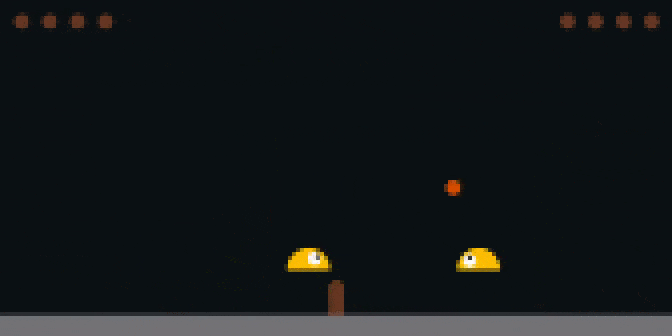
\includegraphics[width=0.8\textwidth]{img/slimevolley.png}
\end{figure}

Second environment is a \emph{Cartpole-swingup} environment. It is inspired by classic reinforcement learning benchmark task, pole-balancing. In this task one end of a pole is attached to a card which moves left and right and the goal is to keep the pole upright. In the original the episode ends when the pole is tilted too much off its neutral position. However in this version the pole is able to rotate $360^\circ$ and the episode ends only if the cart goes out of bounds or 1000 timesteps goes past.

The physics of the pole is controlled by equations specified for "Pendullum Swing-up" in PILCO software package \cite{pilco2013}. Reward is given based on how far is the cart from centre (closer is better) and what is the angle of the pole (more upright is better). State is represented with a 4-entry vector containing the position of the cart, its velocity, sine and cosine of the pole's angle and its angular velocity while action is a number from -1 to 1 which represents force which is applied, in either direction, to the cart.

\begin{figure}[h]
    \caption{Screenshot of Cartpole-swingup environment}
    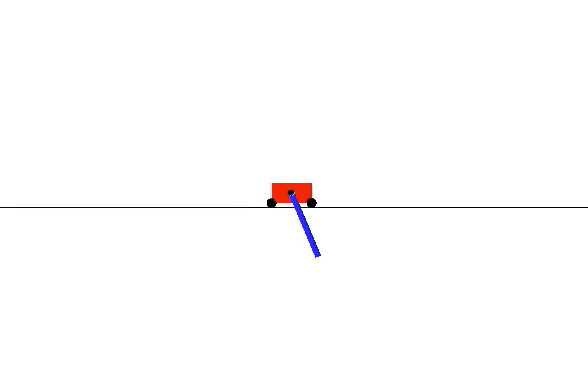
\includegraphics[width=0.8\textwidth]{img/cartpole.png}
\end{figure}
% 
The behavioural characteristics is calculated similarly in both environments, inspired by approach used in \cite{Inden2013} for classic Cartpole problem. For Slimevolley the $x$-coordinate of the controlled agent at timesteps 10, 30, 100, 300, 1000 and 3000 is taken and in Cartpole environment the $x$-coordinate of the cart at timesteps 5, 10, 50, 100, 500 and 100 is taken. If the environment doesn't reach that state a 0 is filled in. This slightly differs from the implementation outlined in \cite{Inden2013}. Then simple Euclidean norm is used to calculcate distance between two such characteristics.

Controlled agents's policies are represented with small feed-forward neural networks, for Cartpole 1-layer neural network with 5 inputs, 10 neurons in middle layer and one output neuron and $\tanh$ activation function applied to output of all neurons. Slimevolley has a bigger network, 12 input neurons, two layers with 20 neurons and 3 output neurons with $\tanh$ activation function. 

\section{Experiments}

There were several experiments run in each environment. All experiments were run 10 times with different starting seeds for 1000 or 900 (in case of novelty based algorithms due to memory contraint on system where experiments were run) generations with population of 90 and 3 episodes per evaluation. The 6 six methods that were tried are:
\begin{itemize}
    \item CMA-ES, 
    \item PEGP,
    \item OpenAI ES,
    \item NS-ES, 
    \item NSR-ES and
    \item NSRA-ES.
\end{itemize}

For CMA-ES, the only parameter was $\sigma_{init}$ which controls the initial standard deviation and it was set to 0.1. PGPE had $\sigma_{init}$ 0.1 and other parameters controlling the standard deviation set to 0.2, 0.999, 0.01 and 0.2 for learning rate, rate of decay, limit and maximal change. OpenAI-ES started with $\sigma$ 0.1, rate of decay 0.999 and limit 0.01. Novelty search based algorithm had fixed $\sigma$ (because it doesn't make sense to change it since there are more individuals) of 0.1 and used 5 as $k$ in k-nearest neighbours and metapopulation with size 5. In addition to that NSRA-ES waited 10 steps before increasing the ratio of novelty in the gradient by 0.05. All algorithms, except for CMA-ES, used the Adam \cite{kingma2017adam} optimiser, with learning rate 0.1. In all presented graphs a median is shown along with the first and third quartile.

\subsection{Slimevolley}

The experiments have shown that this environment is quite challenging to solve. Only CMA-ES has managed to get good results in the 10 runs included in the experiment. Since the reward received by CMA-ES caps at 30 it would suggest that the agent didn't learn to beat the opponent but only to defend well enough. However during development OpenAI-ES has managed to get some good results as well but it was strongly sensitive to seed, equalling the performance of CMA-ES in some runs while not improving at all in others. Novelty search-based methods did fail as well on this problem while intuitively they should have a higher chance of producing good results as they are able to explore in multiple directions at once thus have higher probability of going in the right direction. Bad performance by NS-ES was expected and in accordance with \cite{conti2018}. However both NSR-ES and NSRA-ES did not perform well either which points to either badly designed novelty or suboptimal hyperparameter setting. 

\begin{figure}[H]
    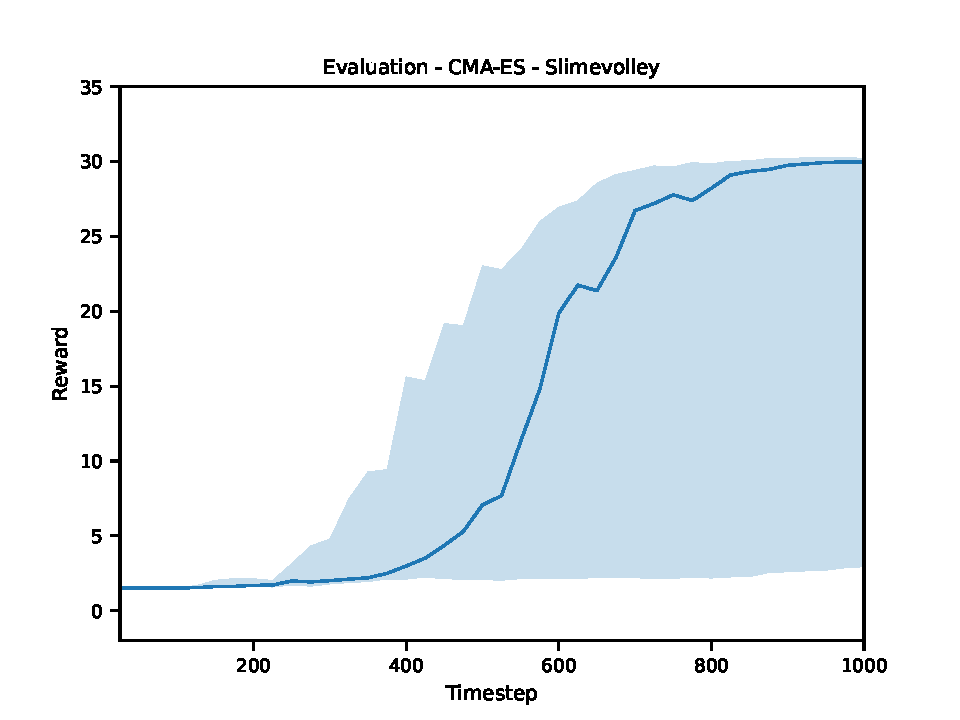
\includegraphics[width=0.9\textwidth]{img/eval-slime-cmaes.pdf}
\end{figure}
\begin{figure}[H]
    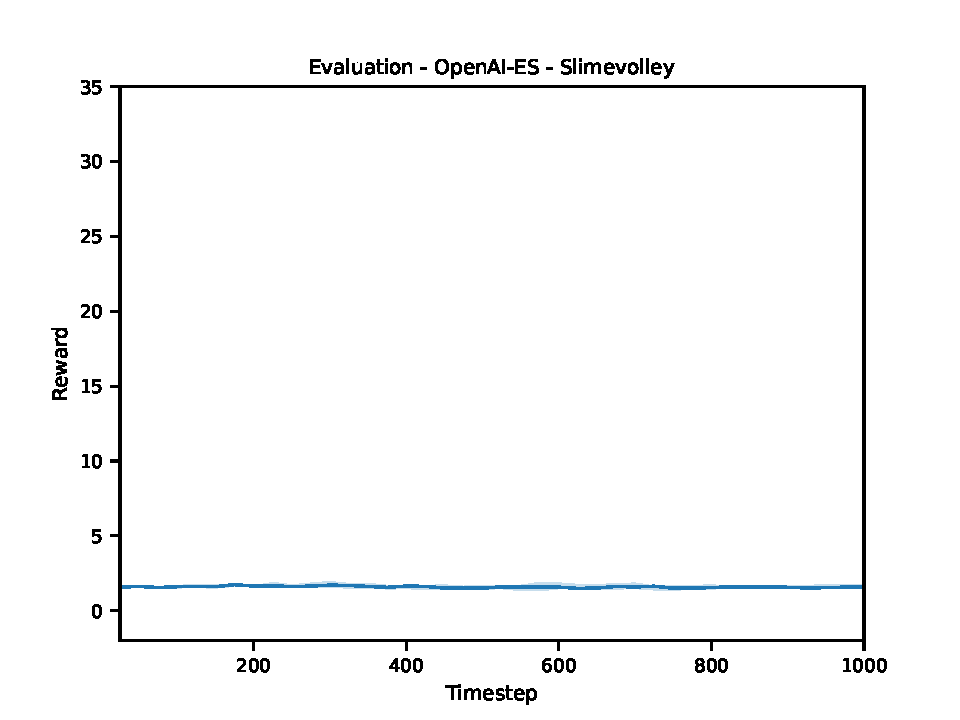
\includegraphics[width=0.9\textwidth]{img/eval-slime-open.pdf}
\end{figure}
\begin{figure}[H]
    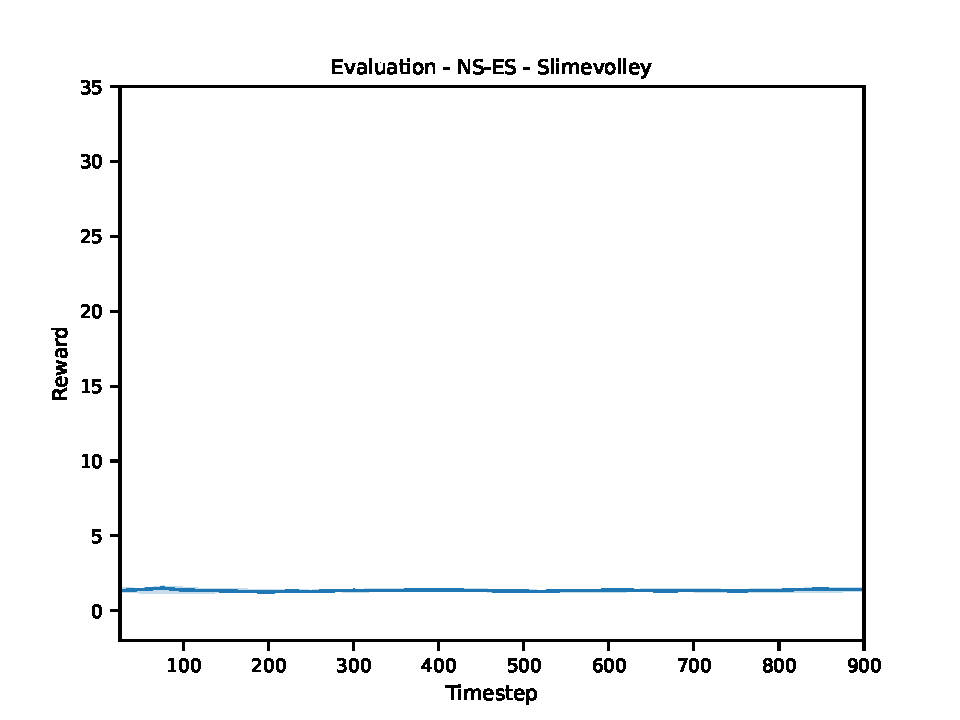
\includegraphics[width=0.9\textwidth]{img/eval-slime-nses.pdf}
\end{figure}
\begin{figure}[H]
    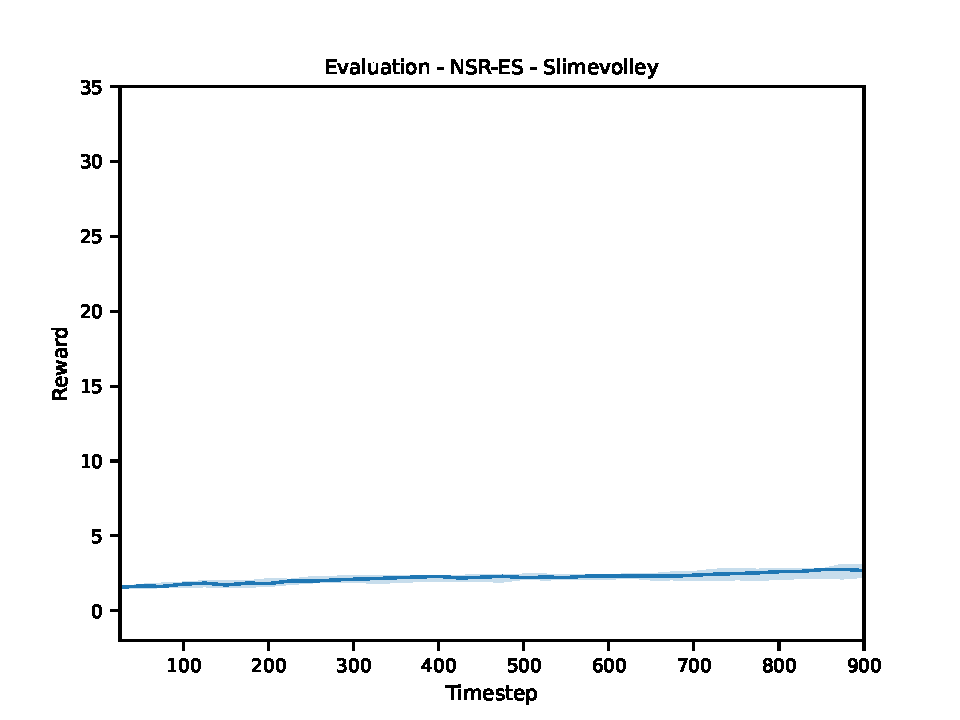
\includegraphics[width=0.9\textwidth]{img/eval-slime-nsres.pdf}
\end{figure}
\begin{figure}[H]
    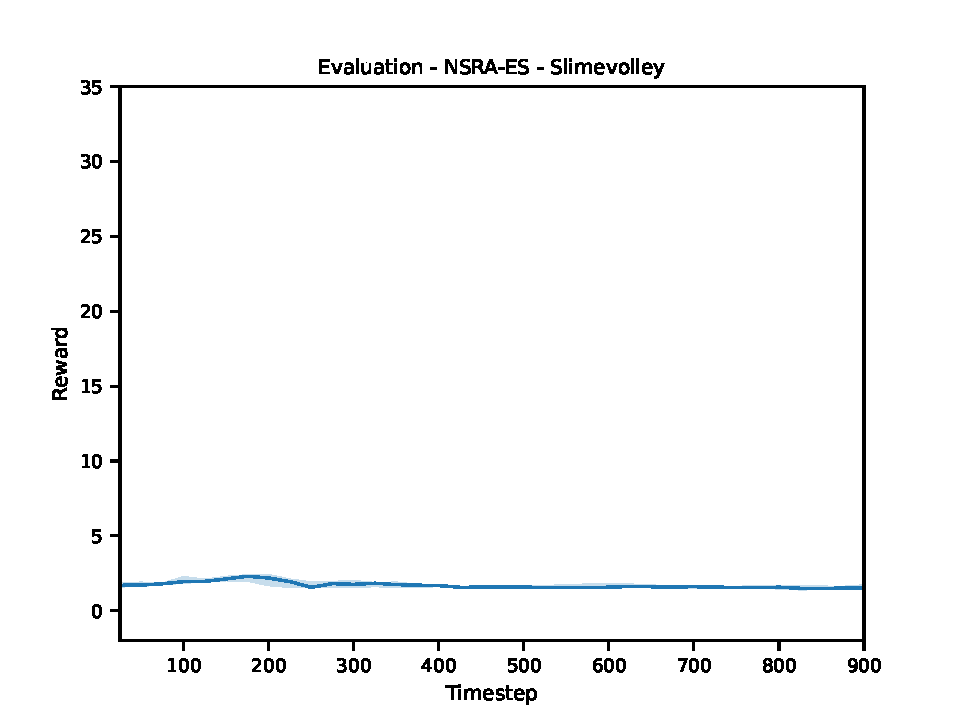
\includegraphics[width=0.9\textwidth]{img/eval-slime-nsraes.pdf}
\end{figure}
\begin{figure}[H]
    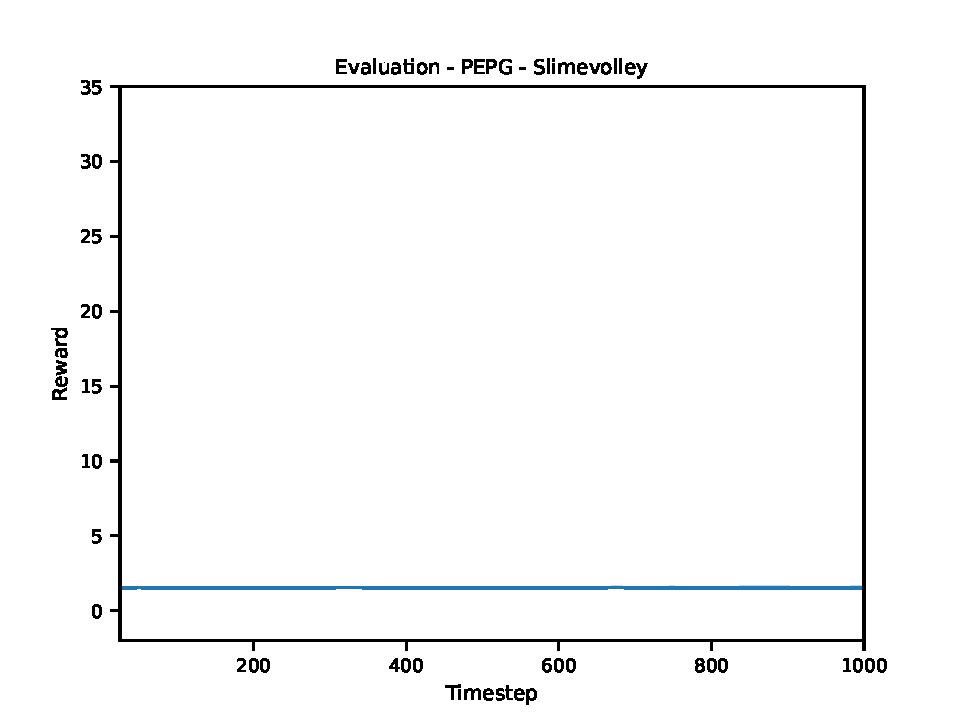
\includegraphics[width=0.9\textwidth]{img/eval-slime-pepg.pdf}
\end{figure}
\newpage

\subsection{Cartpole-swingup}

This environment has proven to be significantly less challenging than Slimovolley. Both OpenAI-ES and CMA-ES have managed to solve it but CMA-ES seems to have a significant performance dropoff in later generations. Closer inspection of data from traning has shown that in some cases the trainig gets stuck at values around 925 with parameters slowly growing in magnitude before completely exploding and performance dropping off. Bad performance from NS-ES was expected as it has no incetive to pursue better performance. NSR-ES slowly and steadily improves and the trajectory suggests that it would improve further given more time. This is most likely thanks to having 1:1 ratio of fitness and novelty therefore the the search for novelty slows down the search for improvement. In case of NSRA-ES a fast improvement can be seen in the beginning however as the weight of novelty slowly increases the algorithm starts to perform similarly to NS-ES. This behaviour can be probably avoided with either better hyperparameter tuning or better novelty calculation.


\begin{figure}[H]
    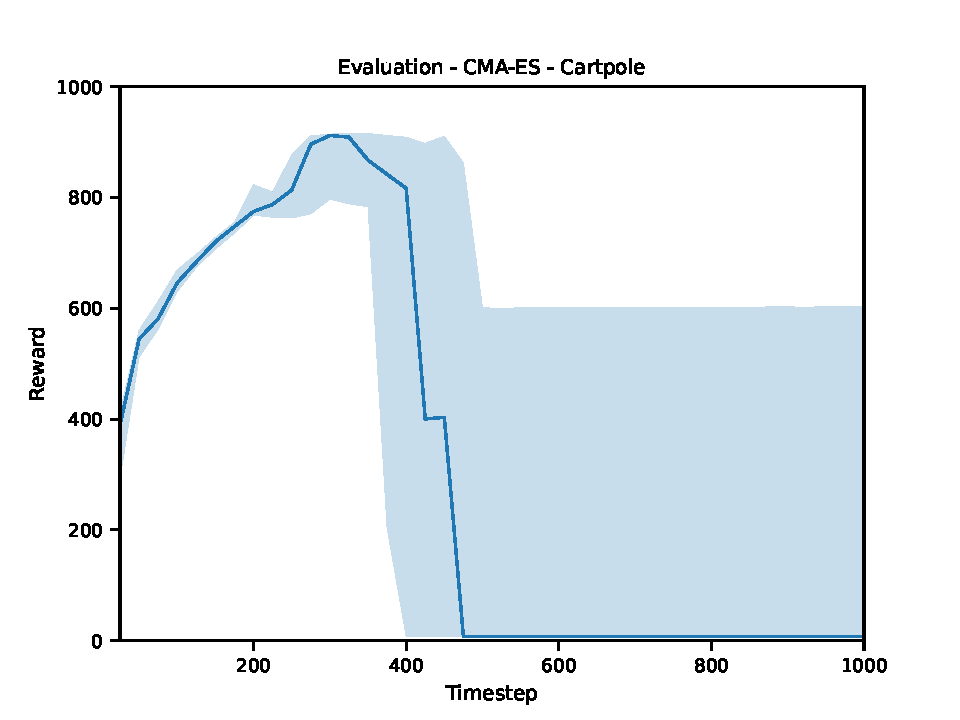
\includegraphics[width=0.9\textwidth]{img/eval-cart-cmaes.pdf}
\end{figure}
\begin{figure}[H]
    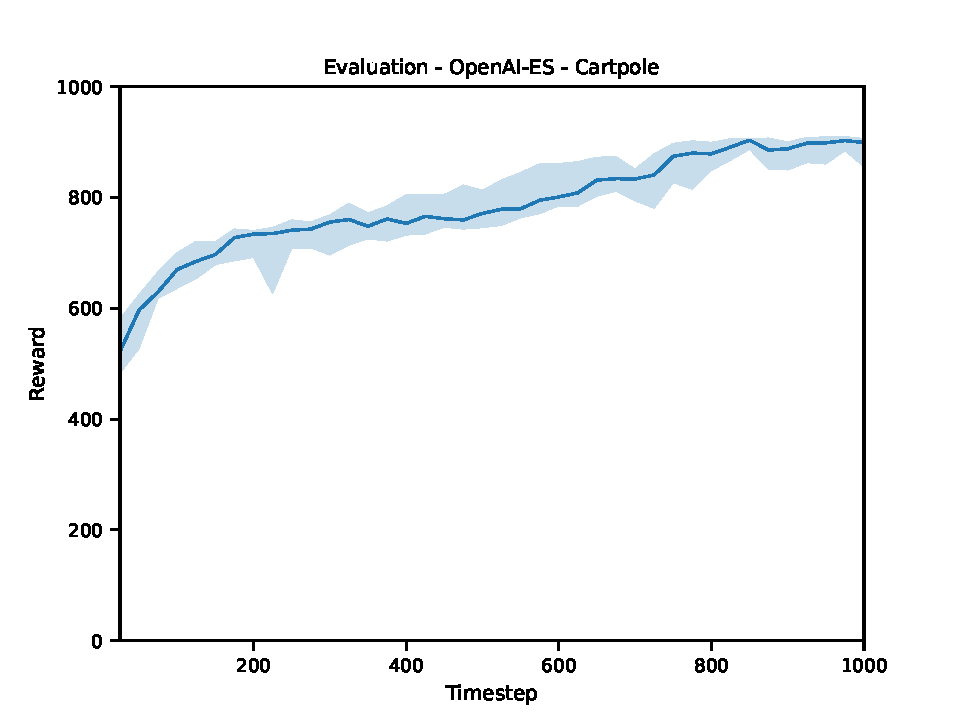
\includegraphics[width=0.9\textwidth]{img/eval-cart-open.pdf}
\end{figure}
\begin{figure}[H]
    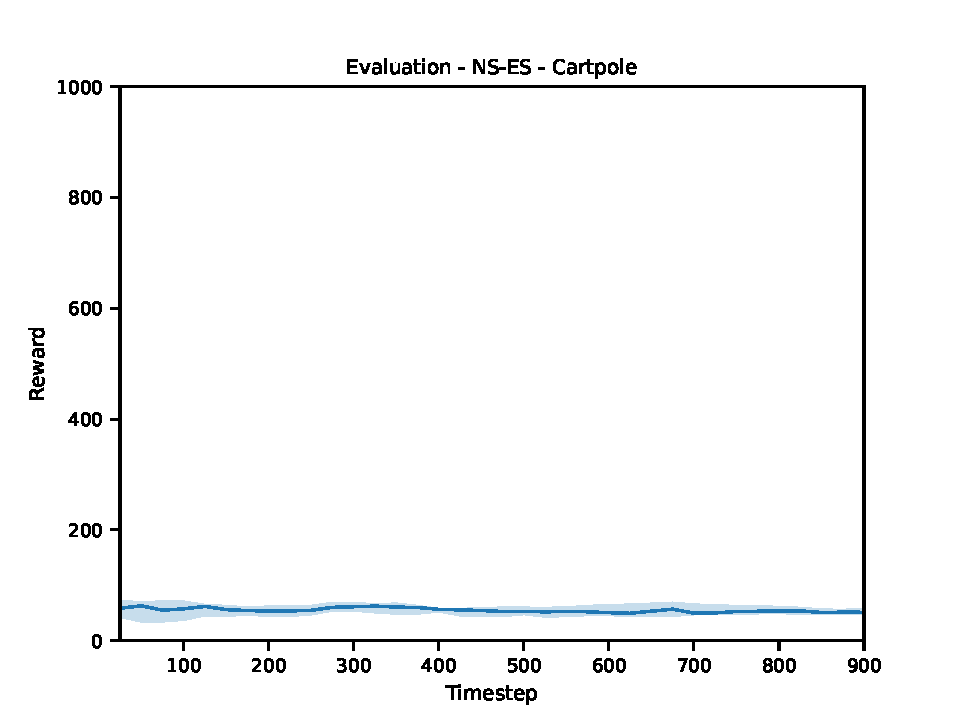
\includegraphics[width=0.9\textwidth]{img/eval-cart-nses.pdf}
\end{figure}
\begin{figure}[H]
    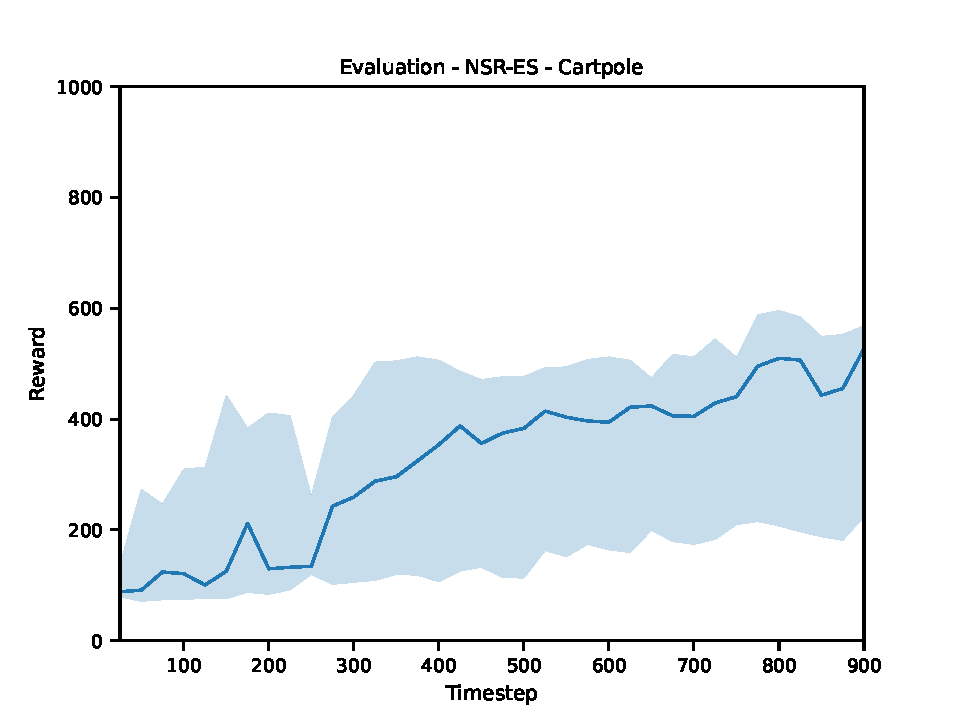
\includegraphics[width=0.9\textwidth]{img/eval-cart-nsres.pdf}
\end{figure}
\begin{figure}[H]
    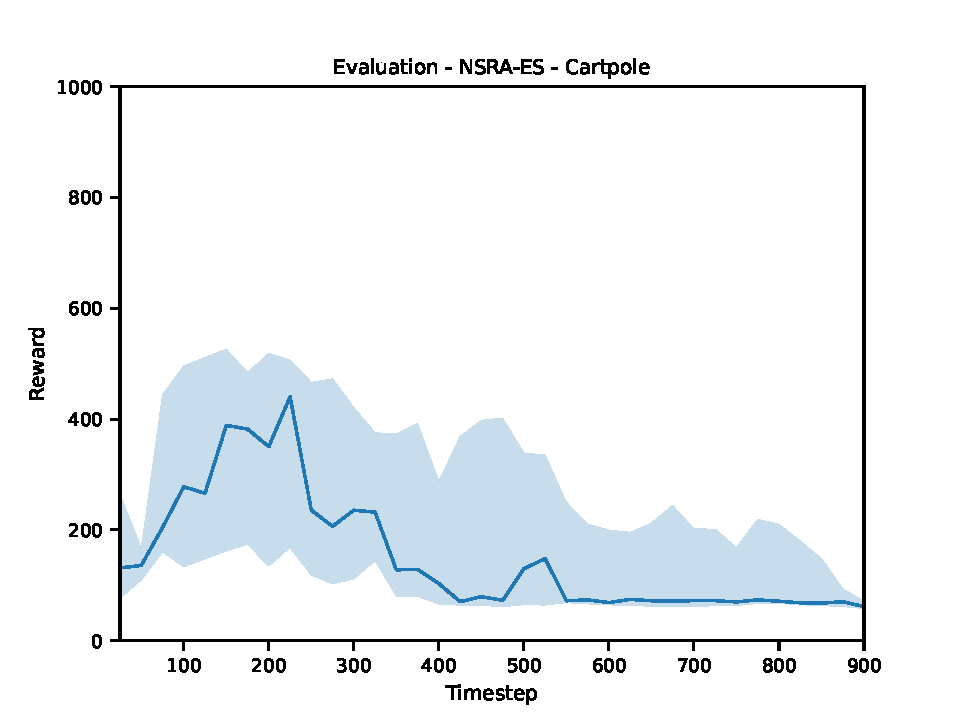
\includegraphics[width=0.9\textwidth]{img/eval-cart-nsraes.pdf}
\end{figure}
\begin{figure}[H]
    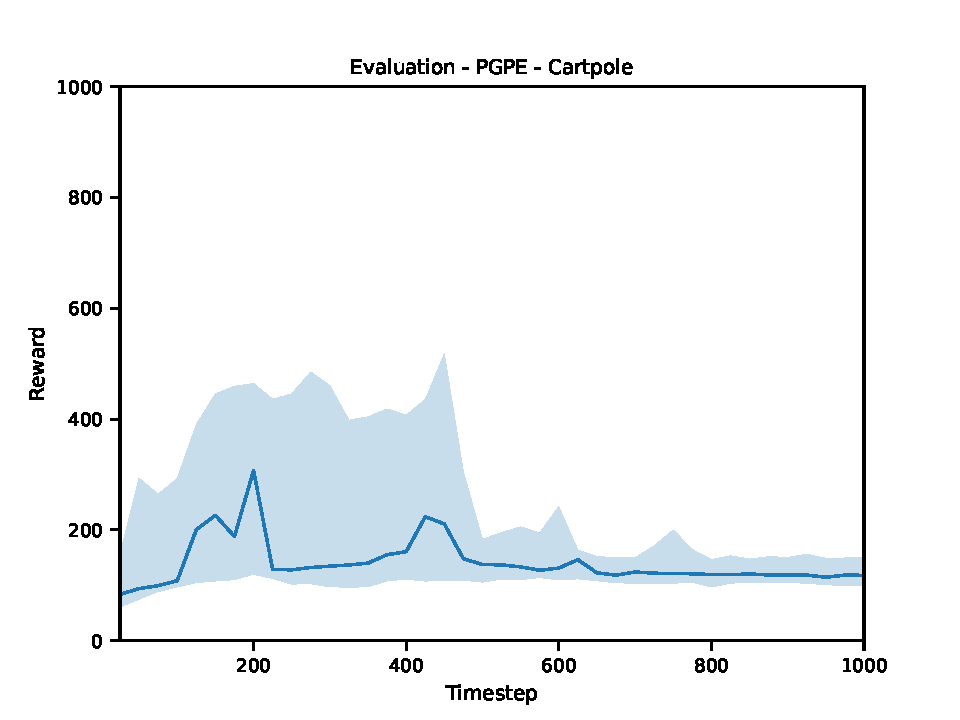
\includegraphics[width=0.9\textwidth]{img/eval-cart-pepg.pdf}
\end{figure}


\chapwithtoc{Conclusion}

In this thesis reinforcement learning was formally introduced along with several methods such as Q-learning or REINFORCE. Then evolutionary algorithms were described and further expanded by evolutionary strategies including the introduction of CMA-ES. Following that OpenAI-ES was outlined, a evolutionary strategy that was designed for solving reinforcement learning tasks, high level of paralellisation and doesn't require differentiable policy as there is no differentiation needed unlike in traditional methods such as REINFORCE. This algorithm is further extended with novelty search which uses behavioral characteristics of evolved agents to evolve agents to behave in a different manner than their ancestors which should enable the agents to deal with falling into a local optima. Then the 2 test environment were outlined and data from experiments discussed. Finally some technical details about the implementation were explained.

Based on conducted experiments Slimevolley is a task that is hard to solve since only one method (CMA-ES) managed to do so and OpenAI-ES did so only few times and the performance varied heavily with seed. Cartpole has proven to be slightly easier with more methods being successful or would succeed given more time. Furthermore novelty search-based algorithm were found to be sensitive to quality of novelty calculation.

This work has shown that designing novelty search-based algorithms is mostly designing a good behavioral characteristic of an agent. Therefore this would be, along with more hyperparameter tuning, a possible direction to follow in research. Furthermore exploring performance of these methods on more environments would be beneficial as well. To get more accurate results on the two environments presented, spending more time with hyperparameter tuning and trying running longer experiments with a bigger population would help. Running more runs for each experiment would also be beneficial as it would create batter





\ifEN
\chapwithtoc{Bibliography}
\else
\chapwithtoc{Seznam použité literatury}
\fi

\printbibliography[heading=none]


\appendix



% if your attachments are complicated, describe them in a separate appendix
%\include{attachments}

\openright
\end{document}
